%!TEX root = ../masters_thesis.tex

\section{Editing Hivent Data} % (fold)
\label{sec:editing_hivent_data}

The previous section explained the abstract Hivent Model, a set of Hivent operations and a promising visualization method. However, one purpose of the HGIS developed in this thesis is to add, alter and delete historical changes. This section presents tools and methods to edit spatio-data in the Hivent Model.

Whereas the Hivent Operations are well-defined and specific, user studies have shown that they are not well understood by humans editing data in the system. This thesis therefore proposes a different set of six \emph{Edit Operations} in section \ref{sub:edit_operations}. Afterwards, section \ref{sub:edit_workflow} introduces a \emph{workflow} to create the data for an Edit Operation step by sep. The main use case of event-based spatio-temporal data models is to append changes to the end of time. But the Hivent Mode also needs to support adding historical changes in between. The last section \ref{sub:retrospective_updates} explains the theoretical approach to \emph{retrospecitve updates} of spatio-temporal data in the Hivent Model.


% ------------------------------------------------------------------------------
\subsection{Edit Operations} % (fold)
\label{sub:edit_operations}

The Hivent Operations are valuable, because they can describe all possible changes in the evolution of countries in time and space. They are really well understood from the system point of view and are therefore the basis for the Hivent Model. However, the purpose of the HGIS developed in this thesis is to provide a well understood user interface to introduce historical changes to countries. Throughout the development process, interviews with historians and other researchers in humanities at University of Virginia were conducted, to understand their mental model about the task. In the interviews it turned out that the Hivent Operations are not suitable to be used for human edit purposes, because of their low-level nature. One example is that the operations do not provide a straightforward way to create a new country on previously unclaimed land. The same is true for changing the formal name of an Area.

Therefore, this thesis introduces a second set of operations: five high-level \emph{Edit Operations} describe changes to countries on the map (see table \ref{tab:edit_operations}). They have proven to be understandable in several user studies.

\begin{table}[H]
\begin{center}
\begin{tabular}{m{0.75cm} m{0.8cm} m{2.4cm} m{9.1cm}}
  \raisebox{-0.35\height}
  {
\includegraphics[width=0.72cm]{graphics/development/edit_operations/CRE}} &
  \texttt{CRE} & Create &
  a new Area with a new name and territory on the map. \\

  \raisebox{-0.35\height}
  {
\includegraphics[width=0.72cm]{graphics/development/edit_operations/MRG}} &
  \texttt{MRG} & Merge &
  two or more Areas to a new Area. The name has to be set manually, the territory is automatically unified. \\

  \raisebox{-0.35\height}
  {
\includegraphics[width=0.72cm]{graphics/development/edit_operations/DIS}} &
  \texttt{DIS} & Dissolve &
  one Area into two or more new Areas, manually setting their new territory and name. \\

  \raisebox{-0.35\height}
  {
\includegraphics[width=0.72cm]{graphics/development/edit_operations/CHB}} &
  \texttt{CHB} & Change Borders &
  between two neighboring Areas by defining the territory that changes sides. \\

  \raisebox{-0.35\height}
  {
\includegraphics[width=0.72cm]{graphics/development/edit_operations/REN}} &
  \texttt{REN} & Rename &
  an Area and set a new formal name, short name or both. \\

  \vspace{0.35em}
  \raisebox{-0.35\height}
  {
\includegraphics[width=0.72cm]{graphics/development/edit_operations/CES}} &
  \texttt{CES} & Cease &
  an Area by deleting it from the map, leaving unclaimed land. \\

\end{tabular}
\caption{The six Edit Operations}
\label{tab:edit_operations}
\end{center}
\end{table}

% - - - - - - - - - - - - - - - - - - - - - - - - - - - - - - - - - - - - - - -
\paragraph{Change direction} % (fold)
\label{par:change_direction}

An important issue is the difference between a \emph{forward} and a \emph{backward change}. The general idea of the Hivent Model is to start at one initial time point $t_0$ and to consecutively add historical changes at time points $t_i > t_0$ that manipulate the current state into the future. A state is invariant until a new historical change is inserted that manipulates it again. For researching purposes this is not suitable, because the current state $t_c: t_c > t_0$ of the map is known. The problem is to describe states in the past. For this purpose the concept of a backward change comes into play: An historical change that manipulates a set of old Areas to a set of new Areas is inserted at time point $t_i$, but into the past ($ t_0 < t_i < t_c$). As an example: Given the initial state 10.06.2016 with present-day Germany created on 03.10.1990 on the map. The user wants to enter the German Reunification. The interface must support separating Germany into East and West, but indicating that this was the state \emph{before} 1990 and the original state was \emph{after} this date. This is complicated, because the conceptual, data and computational model have to support it.

% paragraph change_direction (end)

% - - - - - - - - - - - - - - - - - - - - - - - - - - - - - - - - - - - - - - -
\paragraph{Inverse operations} % (fold)
\label{par:inverse_operations}

Related to this problem is the fact that just like the Hivent Operations in the previous section, also the Edit Operations have inverses: A \texttt{CRE} can be inverted with a \texttt{CES} and a \texttt{MRG} with a \texttt{DIS} operation. \texttt{CHB} and \texttt{REN} can be inverted with themselves,

% paragraph inverse_operations (end)

% - - - - - - - - - - - - - - - - - - - - - - - - - - - - - - - - - - - - - - -
\paragraph{Error correction} % (fold)
\label{par:error_correction}

Correcting wrong information in an event-based system is important to understand: Given time point $t_y$ and an Area $A$ with the name $X$. If $X$ happens to be wrong, it means that the historical change at time point $t_x: t_x < t_y$ that created the name $X$ into Area $A$ is erroneous and has be corrected. Correcting a state means correcting the event that created this state.


% paragraph error_correction (end)

% subsection edit_operations (end)

% ------------------------------------------------------------------------------
\subsection{Edit Workflow} % (fold)
\label{sub:edit_workflow}

The conceptual model of the interface promotes six Edit Operations, introduced in section \ref{sub:edit_operations}. They describe one historical change that transforms a set of old areas into a set of new areas, using internally the Hivent Operations (see section \ref{sub:hivent_operations}). In the interface, the historical change is prepared in a workflow of four steps:

\begin{enumerate}
  \item \texttt{SELECT\_OLD\_AREAS}: The user selects the old Areas that will be changed in the Edit Operation.
  \item \texttt{CREATE\_NEW\_TERRITORIES}: For each new Area resulting from the Edit Operation, the user creates a polypolygon describing the territory of the Area.
  \item \texttt{CREATE\_NEW\_NAMES}: Afterwards the user writes the name of each new Area directly on the map. This finalizes the set of new Areas for the historical change.
  \item \texttt{ADD\_CHANGE}: Finally, the historical change has to be added to an Hivent that introduces it and inherits the time point to it. The user either selects an existing Hivent or creates a new one. All the information necessary for the spatio-temporal Hivent Model are completed.
\end{enumerate}

For each Edit Operation, the requirements for the steps are different. Not all operations need all steps and some data is processed automatically. Table \ref{tab:editoperations_in_worklow} presents an overview about the behaviour of each operation in the first three steps. The last step is the same for each operation: Each historical change has to be added to an Hivent.

\begin{table}[H]
\begin{center}
\begin{tabular}{m{0.9cm} m{4.0cm} m{4.4cm} m{3.8cm}}
  \toprule

  &
  \texttt{SELECT\_OLD\_AREAS} &
  \texttt{CREATE\_NEW\_TERRITORIES} &
  \texttt{CREATE\_NEW\_NAMES} \\

  \midrule
  \texttt{CRE} &
  -- &
  \pbox{4.4cm}{create a territory of the new country\\
  \footnotesize{on unclaimed land and/or overlapping existing countries}} &
  create a name of the new country \\

  \midrule
  \texttt{MRG} &
  select the countries to be merged &
  \pbox{4.4cm}{--\\
  \footnotesize{automatic unification of territories of selected countries}} &
  create a name of the merged country
  \\

  \midrule
  \texttt{DIS} &
  select a country to be \mbox{dissolved} &
  create a territory for each new country &
  create a name for each new country \\

  \midrule
  \texttt{CHB} &
  select two neighboring countries to change their border &
  \pbox{4.4cm}{create the new border between both countries \\
  \footnotesize{the territory for both countries will be created automatically}}  &
  -- \\

  \midrule
  \texttt{REN} &
  select a country to change its name &
  -- &
  create a new name of the country \\

  \midrule
  \texttt{CES} &
  select a country to cease it &
  -- &
  -- \\

  \bottomrule
\end{tabular}
\caption{The requirements of each step for the Edit Operations}
\label{tab:editoperations_in_worklow}
\end{center}
\end{table}


% - - - - - - - - - - - - - - - - - - - - - - - - - - - - - - - - - - - - - - -
\paragraph{Edit Operations to Hivent Operations} % (fold)
\label{par:edit_operations_to_hg_operations}

% wording:
% UNI of "[old]"  to    "new"
% INC of "[old]"  into  "pres"
% SEP of "old"    into  "[new]"
% SEC of "[new]"  from  "pres"
% NCH of "pres"

The six high-level Edit Operations can be expressed by a combination of the and the five low-level Hivent Operations. Depending on the input of the user in the Edit Operation steps, there are different possibilities. They are introduced in table \ref{tab:editoperations_to_hg_operations}.

Hivent Operations can be combined when they happen at the same time, e.g. if one Area incorporates another Area and thereby changes its short name, this is a combination of \texttt{INC + NCH}. When West Germany incorporated East Germany in 1900, it was from that moment on just called Germany.


\newpage
\begin{center}
\begin{longtable}{m{1.2cm} m{0.95cm} m{0.95cm} m{0.95cm} m{6.0cm} m{2.3cm}}
  \toprule

  \pbox{1.2cm}{EditOp.\\(case)} &
  \pbox{0.95cm}{old\\Areas\\[-0.8em]} &
  \pbox{0.95cm}{update\\Areas\\[-0.8em]} &
  \pbox{0.95cm}{new\\Areas\\[-0.8em]} &
  expression by Hivent Operations \protect\footnotemark &
  visualization \\
  \midrule
  \endhead

  % TODO: introduce T as territory that is used like a temporary Area with exactly that territoy
  % CREATE

  \multirow{9}{*}{\texttt{CRE} (1)} &
  \multicolumn{4}{p{10cm}}{
    Area $B_1$ is created with territory $T$. The part of $T$ that is on previously unclaimed land ($T_\Omega$) is seceded as $B_1$ from $\Omega$.
    If $T_\Omega$ is empty, then $B_1$ is initialized with an empty territory.
    The rest of $T$ covers some Areas $A_p$ partially and some Areas $A_f$ fully.
    For each $A_p$, the covered territory $T_p$ is seceded and incorporated into $B_1$.
    Each $A_f$ is completely incorporated into $B_1$.
  } &
  \multirow{9}{*}{
    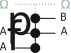
\includegraphics[width=2.5cm]{graphics/development/edit_to_hg_operations/CRE_to_SEC+UNI}
  } \\

  &
  $n_f$ &
  $n_p$ &
  $1$ &
  \pbox{6.0cm}{
    ~\\
    \texttt{SEC} of $B_1$ from $\Omega$ \\
    \texttt{SEC} of $T_p$ from $A_p$, \texttt{INC} of $T_p$ into $B_1$ \\
    \texttt{INC} of $A_f$ into $B_1$
  } &
  \\

  % MERGE
  \midrule
  \multirow{3}{*}{\texttt{MRG} (1)} &
  \multicolumn{4}{p{10cm}}{
    Multiple Areas $A_i$ are unified to $B_1$. The new Area receives a new name distinct from all the names of $A_i$.
  } &
  \multirow{3}{*}{
    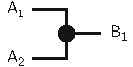
\includegraphics[width=2.5cm]{graphics/development/edit_to_hg_operations/MRG_to_UNI}
  } \\
  &
  $n \geq 2$ &
  $0$ &
  $1$ &
  \pbox{6.0cm}{
    ~\\
    \texttt{UNI} of $\forall A_i$ to $B_1$
  } &
  \\

  \midrule
  \multirow{4}{*}{\texttt{MRG} (2)} &
  \multicolumn{4}{p{10cm}}{
    Multiple Areas $A_i$ are unified, the resulting Area reuses the short and formal name of one of the old Areas ($A_p$) and therefore preserves it. The remaining Areas $A_i$ are incorporated into $A_p$.
  } &
  \multirow{4}{*}{
    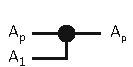
\includegraphics[width=2.5cm]{graphics/development/edit_to_hg_operations/MRG_to_INC}
  } \\
  &
  $n \geq 1$ &
  $1$ &
  $1$ &
  \pbox{6.0cm}{
    ~\\
    \texttt{INC} of $\forall A_i$ into $A_p$
  } &
  \\

  \midrule
  \multirow{4}{*}{\texttt{MRG} (3)} &
  \multicolumn{4}{p{10cm}}{
    The same as the previous case, just that $A_p$ receives a new short name and therefore an additional name change is required.
  } &
  \multirow{4}{*}{
    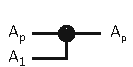
\includegraphics[width=2.5cm]{graphics/development/edit_to_hg_operations/MRG_to_INC+NCH}
  } \\
  &
  $n \geq 1$ &
  $1$ &
  $1$ &
  \pbox{6.0cm}{
    ~\\
    \texttt{INC} of $\forall A_i$ into $A_p$ \\
    \texttt{NCH} of $A_p$
  } &
  \\

  % DISSOLVE

  \midrule
  \multirow{4}{*}{\texttt{DIS} (1)} &
  \multicolumn{4}{p{10cm}}{
    Separate one Area $A_1$ into multiple new Areas $B_i$ and define a territory and name for each of them. Each name is distinct from the name of the old Area.
  } &
  \multirow{4}{*}{
    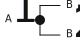
\includegraphics[width=2.5cm]{graphics/development/edit_to_hg_operations/DIS_to_SEP}
  } \\
  &
  $1$ &
  $0$ &
  $n \geq 2$ &
  \pbox{6.0cm}{
    ~\\
    \texttt{SEP} of $A_1$ into $\forall B_i$
  } &
  \\

  \midrule
  \multirow{5}{*}{\texttt{DIS} (2)} &
  \multicolumn{4}{p{10cm}}{
    Separate multiple Areas $B_1$ from one initial Area $A_p$ and define a territory and name for each of them. One of the separated Areas has the same short and formal name as $A_p$, so it continues its identity and preserves the Area. The remaining new Areas secede from $A_p$.
  } &
  \multirow{5}{*}{
    
\includegraphics[width=2.5cm]{graphics/development/edit_to_hg_operations/DIS_to_SEC}
  } \\
  &
  $1$ &
  $1$ &
  $n \geq 1$ &
  \pbox{6.0cm}{
    ~\\
    \texttt{SEC} of $\forall B_i$ from $A_p$
  } &
  \\

  \midrule
  \multirow{4}{*}{\texttt{DIS} (3)} &
  \multicolumn{4}{p{10cm}}{
    The same as the previous case, just that $A_p$ receives a new short name and therefore an additional name change is required.
  } &
  \multirow{4}{*}{
    
\includegraphics[width=2.5cm]{graphics/development/edit_to_hg_operations/DIS_to_SEC+NCH}
  } \\
  &
  $1$ &
  $1$ &
  $n \geq 1$ &
  \pbox{6.0cm}{
    ~\\
    \texttt{SEC} of $\forall B_i$ from $A_p$  \\
    \texttt{NCH} of $A_p$
  } &
  \\

  % CHANGE BORDER

  \midrule
  \multirow{10}{*}{\texttt{CHB} (1)} &
  \multicolumn{4}{p{10cm}}{
    One existing Area $A_1$ is selected and its territory changes. Relative to the old territory some parts of the territory expanded ($T_e$) and some withdrew ($T_w$).
    The part of $T_e$ that expanded into unclaimed land ($T_\Omega \in T_e$) is seceded from $\Omega$ and incorporated into $A_1$.
    The Areas $A_f$ fully covered by $T_e$ are incorporated into $A_1$,
    the Areas $A_p$ partially covered by $T_e$ secede this territory $T_p \in T_e$ to $A_1$.
    $T_w$ will be incorporated into $\Omega$, resulting in unclaimed land.
  } &
  \multirow{10}{*}{
    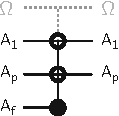
\includegraphics[width=2.5cm]{graphics/development/edit_to_hg_operations/CHB_to_SEC+INC_omega}
  } \\
  &
  $n_f$ &
  $1+n_p$ &
  $0$ &
  \pbox{6.0cm}{
    ~\\
    \texttt{SEC} of $T_\Omega$ from $\Omega$,
    \texttt{INC} of $T_\Omega$ into $A_1$ \\
    \texttt{SEC} of $T_p$ from $A_p$,
    \texttt{INC} of $T_p$ into $B_1$ \\
    \texttt{INC} of $A_f$ into $B_1$ \\
    \texttt{SEC} of $T_w$ from $B_1$,
    \texttt{INC} of $T_w$ into $\Omega$
  } &
  \\

  \midrule
  \multirow{7}{*}{\texttt{CHB} (2)} &
  \multicolumn{4}{p{10cm}}{
    Two existing Areas $A_1$ and $A_2$ are selected and their common border changes. This results in a symmetrical change of territories, made up by two sets of territories: $T_2$ that previously belonged to $A_1$ and is now part of $A_2$ and $T_1$ for which the opposite is true. $T_2$ is seceded by $A_1$ and incorporated into $A_2$, the opposite happenes to $T_1$.
  } &
  \multirow{7}{*}{
    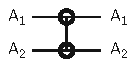
\includegraphics[width=2.5cm]{graphics/development/edit_to_hg_operations/CHB_to_SEC+INC}
  } \\
  &
  $0$ &
  $2$ &
  $0$ &
  \pbox{6.0cm}{
    ~\\
    \texttt{SEC} of $T_2$ from $A_1$,
    \texttt{INC} of $T_2$ into $A_2$ \\
    \texttt{SEC} of $T_1$ from $A_2$,
    \texttt{INC} of $T_1$ into $A_1$
  } &
  \\

  % RENAME

  \midrule
  \multirow{3}{*}{\texttt{REN} (1)} &
  \multicolumn{4}{p{10cm}}{
    One Area $A_1$ is selected and both its short and formal name is changed. Therefore, a new Area $B_1$ is created as a direct successor of $A_1$. This is a special case of a unification with only one Area.
  } &
  \multirow{3}{*}{
    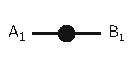
\includegraphics[width=2.5cm]{graphics/development/edit_to_hg_operations/REN_to_UNI}
  } \\
  &
  $1$ &
  $0$ &
  $1$ &
  \pbox{6.0cm}{
    \texttt{UNI} of $A_1$ to $B_1$
  } &
  \\

  \midrule
  \multirow{3}{*}{\texttt{REN} (2)} &
  \multicolumn{4}{p{10cm}}{
    One Area $A_1$ is selected and receives a new short name, but the formal name and therefore the identity is preserved. $A_1$ is updated.
  } &
  \multirow{3}{*}{
    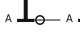
\includegraphics[width=2.5cm]{graphics/development/edit_to_hg_operations/REN_to_NCH}
  } \\
  &
  $0$ &
  $1$ &
  $0$ &
  \pbox{6.0cm}{
    \texttt{NCH} of $A_1$
  } &
  \\

  % CEASE

  \midrule
  \multirow{2}{*}{\texttt{CES} (1)} &
  \multicolumn{4}{p{10cm}}{
    One Area $A_1$ is selected and ceases by incorporating into the universe.
  } &
  \multirow{2}{*}{
    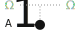
\includegraphics[width=2.5cm]{graphics/development/edit_to_hg_operations/CES_to_INC}
  } \\
  &
  $1$ &
  $0$ &
  $0$ &
  \pbox{6.0cm}{
    \texttt{INC} of $A_1$ into $\Omega$
  } &
  \\

  \bottomrule
\caption{Translation from Edit Operations to Hivent Operations}
\end{longtable}
\label{tab:editoperations_to_hg_operations}
\end{center}
\footnotetext{multiple Hivent Operations in one row happen exactly at the same time point, so they are combined}

% paragraph edit_operations_to_hg_operations (end)

% subsection edit_workflow (end)

% ------------------------------------------------------------------------------
\subsection{Retrospective Updates} % (fold)
\label{sub:retrospective_updates}

% subsection retrospective_updates (end)

% section editing_hivent_data (end)